\documentclass{beamer}
\mode<presentation>
%\usetheme{Warsaw}

\usepackage{amsmath, amssymb, amsthm, graphicx, enumerate, subfigure}
\usepackage{verbatim}
\usepackage[spanish,mexico]{babel}
\usepackage[utf8]{inputenc}
\usepackage[labelformat=empty]{caption}
\usepackage{pifont}% http://ctan.org/pkg/pifont

\definecolor{green1}{rgb}{0.1,0.5,0.2}
\definecolor{green2}{rgb}{0.9,1,0.9}
\definecolor{green3}{rgb}{0.1,0.3,0.2}
\definecolor{green4}{rgb}{0.9,1,0.9}

\useinnertheme{rectangles}


\setbeamercolor*{Title bar}{fg=white, bg=green1}
\setbeamercolor*{section in head/foot}{bg=green1,fg=white}
\setbeamercolor*{title}{fg=white, bg=green1}
\setbeamercolor*{Location bar}{fg=white,bg=green}
\setbeamercolor*{frametitle}{parent=Title bar}
\setbeamercolor*{block title}{bg=green1,fg=white}
\setbeamercolor*{block body}{bg=green2,fg=green3}
\setbeamercolor*{normal text}{bg=white,fg=green3}
\setbeamercolor*{structure}{bg=white,fg=green1}

\newtheorem{defn}{Definición}
\newtheorem{teo}{Teorema}
\newtheorem{prop}{Proposición}

\newcommand{\R}{\mathbb{R}}
\newcommand{\cmark}{\ding{51}}
\newcommand{\xmark}{\ding{55}}

\title{Sistema de recomendación de hoteles similares}
\subtitle{TESIS}
\institute{
\includegraphics[width=0.3\textwidth]{imagenes/logo_ITAM.jpg}\\INSTITUTO TECNOLÓGICO AUTÓNOMO DE MÉXICO}
\author{Felipe Gerard Valdés}
\date{Febrero de 2016}



\AtBeginSection[]
{
	\begin{frame}<beamer>{Agenda}
		\tableofcontents[currentsection]
	\end{frame}
}


\begin{document}

%%%%%%%%%%%%%%%%%%%%%%%%%%%%%%%%%%%%%%%%%%%%%%%%%

\begin{frame}
	\titlepage
\end{frame}

%%%%%%%%%%%%%%%%%%%%%%%%%%%%%%%%%%%%%%%%%%%%%%%%%
\begin{frame}{Agenda}
	\tableofcontents
\end{frame}

%%%%%%%%%%%%%%%%%%%%%%%%%%%%%%%%%%%%%%%%%%%%%%%%%
%%%%%%%%%%%%%%%%%%%%%%%%%%%%%%%%%%%%%%%%%%%%%%%%%
\section{Planteamiento}

%%%%%%%%%%%%%%%%%%%%%%%%%%%%%%%%%%%%%%%%%%%%%%%%%
\begin{frame}{Resumen}
	\begin{itemize}%[<+->]
		\item Modelo implementado en \textbf{Best Day} (agencia de viajes online)
		\item \textbf{Situación inicial:}
		\begin{itemize}
			\item El sistema de recomendación es estático
			\begin{itemize}
				\item Criterio: Destino + Estrellas
			\end{itemize}
			\item Los clientes potenciales no encuentran el hotel que buscan fácilmente
			\item Por lo tanto, pueden abandonar la página o no encontrar la mejor opción para ellos
			\item Esto impacta los KPIs de la empresa
		\end{itemize}
		\item \textbf{Solución propuesta:} Recomendar con un criterio dinámico que tome en cuenta las principales características del hotel seleccionado
	\end{itemize}
\end{frame}

%%%%%%%%%%%%%%%%%%%%%%%%%%%%%%%%%%%%%%%%%%%%%%%%%
\begin{frame}{Análisis de la competencia}
	\begin{itemize}%[<+->] 
		\item Competidores principales: Price Travel, Booking, Despegar, Expedia, Trip Advisor
		\item Diversas formas de recomendar:
		\begin{itemize}
			\item Hoteles recientemente vistos
			\begin{itemize}
				\item[$\rightarrow$] No son recomendaciones genuinas
			\end{itemize}
			\item Hoteles cercanos / en el mismo destino
			\begin{itemize}
				\item[$\rightarrow$] Estilo y precios pueden ser muy distintos
			\end{itemize}
			\item Recomendaciones con métodos desconocidos (p.ej. ``a otros usuarios les gustó...'')
			\begin{itemize}
				\item[$\rightarrow$] Estilo y precios pueden ser muy distintos
			\end{itemize}
		\end{itemize}
	\item \textbf{Conclusión:} La competencia se enfrenta a los mismos retos y no los ha logrado resolver del todo
	\end{itemize}
\end{frame}

%%%%%%%%%%%%%%%%%%%%%%%%%%%%%%%%%%%%%%%%%%%%%%%%%
\begin{frame}{Consideraciones}
	\begin{itemize}%[<+->] 
		\item Evitar mostrar hoteles demasiado caros
		\item Tomar en cuenta el perfil del hotel
		\item Incorporar información geográfica más detallada que el destino
		\item Diseñar un criterio que se adapte a zonas con diferentes densidades de hoteles
		\item Evitar que el sistema se estanque en las mismas recomendaciones (efecto laberinto)
	\end{itemize}
\end{frame}

%%%%%%%%%%%%%%%%%%%%%%%%%%%%%%%%%%%%%%%%%%%%%%%%%
%%%%%%%%%%%%%%%%%%%%%%%%%%%%%%%%%%%%%%%%%%%%%%%%%
\section{Solución}

%%%%%%%%%%%%%%%%%%%%%%%%%%%%%%%%%%%%%%%%%%%%%%%%%
\begin{frame}{Plan de ataque}
	\begin{enumerate}%[<+->] 
		\item \textbf{Precio:} Filtrar hoteles demasiado caros
		\item \textbf{Similitud:} Construir un \textit{criterio integral de similitud}
		\begin{itemize}
			\item Cantidad de servicios
			\item Perfil similar
		\end{itemize}
		\item \textbf{Distancia:} Recomendar hoteles geográficamente cercanos
	\end{enumerate}
\end{frame}

%%%%%%%%%%%%%%%%%%%%%%%%%%%%%%%%%%%%%%%%%%%%%%%%%
\begin{frame}{(1) Precio}
	\begin{itemize}%[<+->] 
		\item Poner hoteles demasiado caros no promueve el interés del cliente
		\item Generalmente más barato es mejor (siempre y cuando tenga la categoría suficiente)
		\item[$\mathbf{\rightarrow}$] Porcentaje máximo arriba del hotel original
		\item Hoteles por encima del precio establecido son invisibles
	\end{itemize}
\end{frame}

%%%%%%%%%%%%%%%%%%%%%%%%%%%%%%%%%%%%%%%%%%%%%%%%%
\begin{frame}{(2) Similitud (P1)}
	\begin{itemize}%[<+->] 
		\item Las estrellas no bastan como medida de similitud entre hoteles porque no toman en cuenta el estilo del hotel
		\item \textbf{Alternativa:} Usar información de servicios
		\item Usarla directamente es ruidoso porque no toma en cuenta sustitutos
		\item \textbf{Solución:} Agrupar los servicios en categorías
		\item \textbf{Método:} Manual (criterio de negocio) + aglomerado jerárquico
		\item \textbf{Resultado:} Cada hotel tiene un vector que lo caracteriza con el número de servicios en cada una de las categorías
	\end{itemize}
\end{frame}

%%%%%%%%%%%%%%%%%%%%%%%%%%%%%%%%%%%%%%%%%%%%%%%%%
\begin{frame}{(2) Similitud (P2)}
	\begin{itemize}%[<+->] 
		\item El siguiente paso es definir una medida de similitud en el espacio de los vectores de características
		\item Hay dos aspectos importantes que queremos controlar:
		\begin{itemize}
			\item \textbf{Servicios:}
			\begin{itemize}
				\item Al menos ciertos servicios ($\sim$ estrellas)
				\item Los servicios faltantes restan similitud
				\item Los servicios extras no se penalizan
			\end{itemize}
			\item \textbf{Perfil:}
			\begin{itemize}
				\item Hoteles del mismo estilo
				\item Misma proporción de cada categoría
				\item Ignorar la cantidad de servicios
				\item Podría dar hoteles más sencillos o más lujosos
			\end{itemize}
		\end{itemize}
	\end{itemize}
\end{frame}

%%%%%%%%%%%%%%%%%%%%%%%%%%%%%%%%%%%%%%%%%%%%%%%%%
\begin{frame}{(2) Similitud (P2)}
	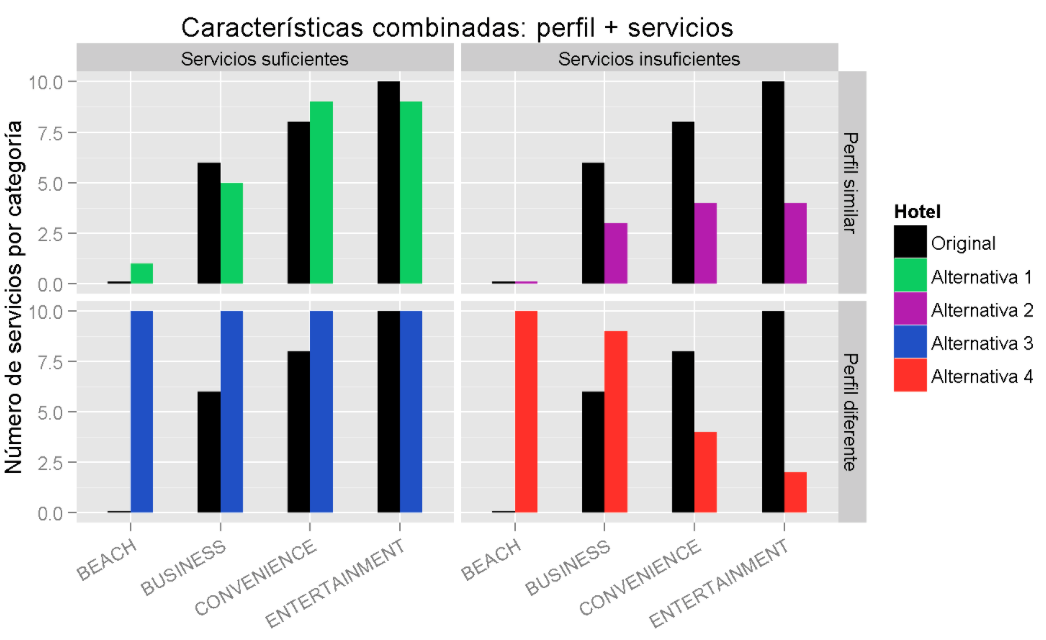
\includegraphics[width=\textwidth]{imagenes/similitud.png}
\end{frame}


%%%%%%%%%%%%%%%%%%%%%%%%%%%%%%%%%%%%%%%%%%%%%%%%%
\begin{frame}{(2) Similitud (P3)}
	\begin{itemize}%[<+->] 
		\item Medida de similitud de servicios: Garantiza que las recomendaciones tengan una cantidad razonable de servicios
		\item Medida de similitud de perfil: Promueve que los hoteles alternativos sean del mismo estilo que el que se está viendo
		\item Medida de similitud final:
		\begin{itemize}
			\item Capturar ambos efectos
			\item Promedio ponderado entre ambas medidas
			\item Ponderación de acuerdo a la variabilidad de cada una (PCA)
		\end{itemize}
		\item ¿Por qué no diferencia absoluta?
		\begin{itemize}
			\item Es simétrica $\implies$ Es demasiado agresiva con los hoteles mejores
			\item No distingue entre perfil y servicios $\implies$ No es ajustable
		\end{itemize}
	\end{itemize}
\end{frame}

%%%%%%%%%%%%%%%%%%%%%%%%%%%%%%%%%%%%%%%%%%%%%%%%%
\begin{frame}{(3) Distancia}
	\begin{itemize}%[<+->] 
		\item Hoteles cercanos (usando coordenadas)
		\item El significado de ``cerca'' depende de la densidad de hoteles en la zona
		\item Se necesita un criterio que se adapte a los cambios de escala
		\item Hay que evitar que los hoteles distintos (pero cercanos) no introduzcan demasiado ruido
	\end{itemize}
\end{frame}

%%%%%%%%%%%%%%%%%%%%%%%%%%%%%%%%%%%%%%%%%%%%%%%%%
\begin{frame}{(3) Distancia}
	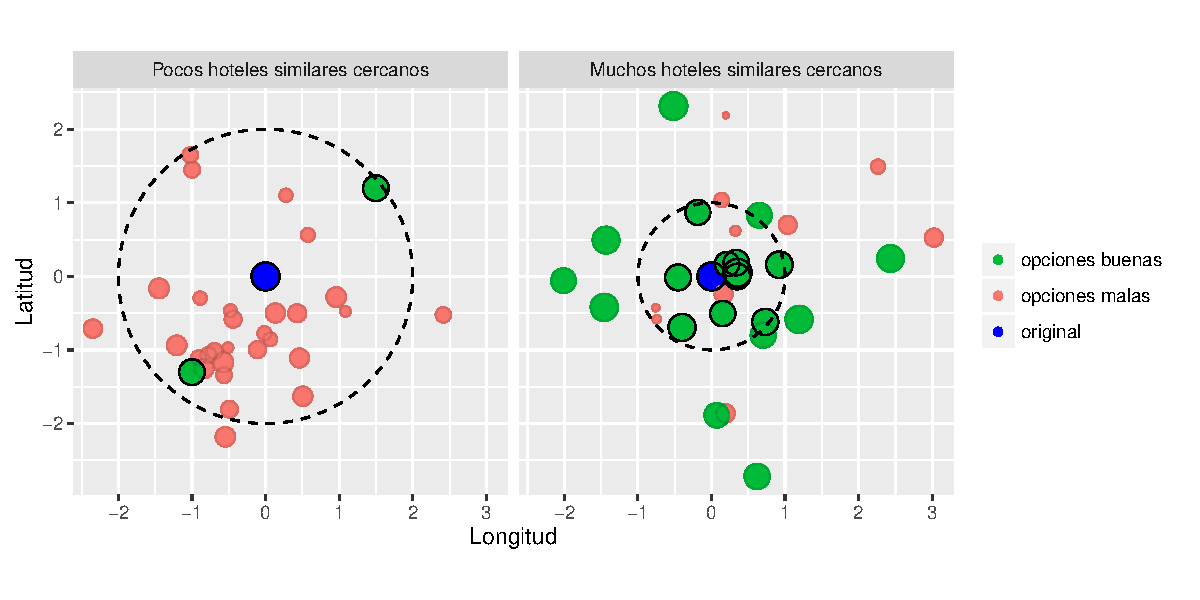
\includegraphics[width=\textwidth]{imagenes/distdin.pdf}
\end{frame}

%%%%%%%%%%%%%%%%%%%%%%%%%%%%%%%%%%%%%%%%%%%%%%%%%
\begin{frame}{Modelo completo}
	\begin{enumerate}%[<+->]
		\item Agrupar los servicios en categorías
		\item Calcular la ponderación entre servicios y perfil
		\item Definir una \textbf{geocerca} (radio de cercanía razonable) alrededor de cada hotel
		\begin{itemize}
			\item Ignorar hoteles caros (precio de largo plazo)
			\item Acumular una cantidad de similitud (mayor peso a hoteles parecidos, menor a los diferentes)
		\end{itemize}
		\item Recomendar dentro de la geocerca de acuerdo a la \textbf{similitud}
	\end{enumerate}
\end{frame}

%%%%%%%%%%%%%%%%%%%%%%%%%%%%%%%%%%%%%%%%%%%%%%%%%
%%%%%%%%%%%%%%%%%%%%%%%%%%%%%%%%%%%%%%%%%%%%%%%%%
\section{Implementación}

%%%%%%%%%%%%%%%%%%%%%%%%%%%%%%%%%%%%%%%%%%%%%%%%%
\begin{frame}{Arquitectura: SQL + \texttt{R}}
	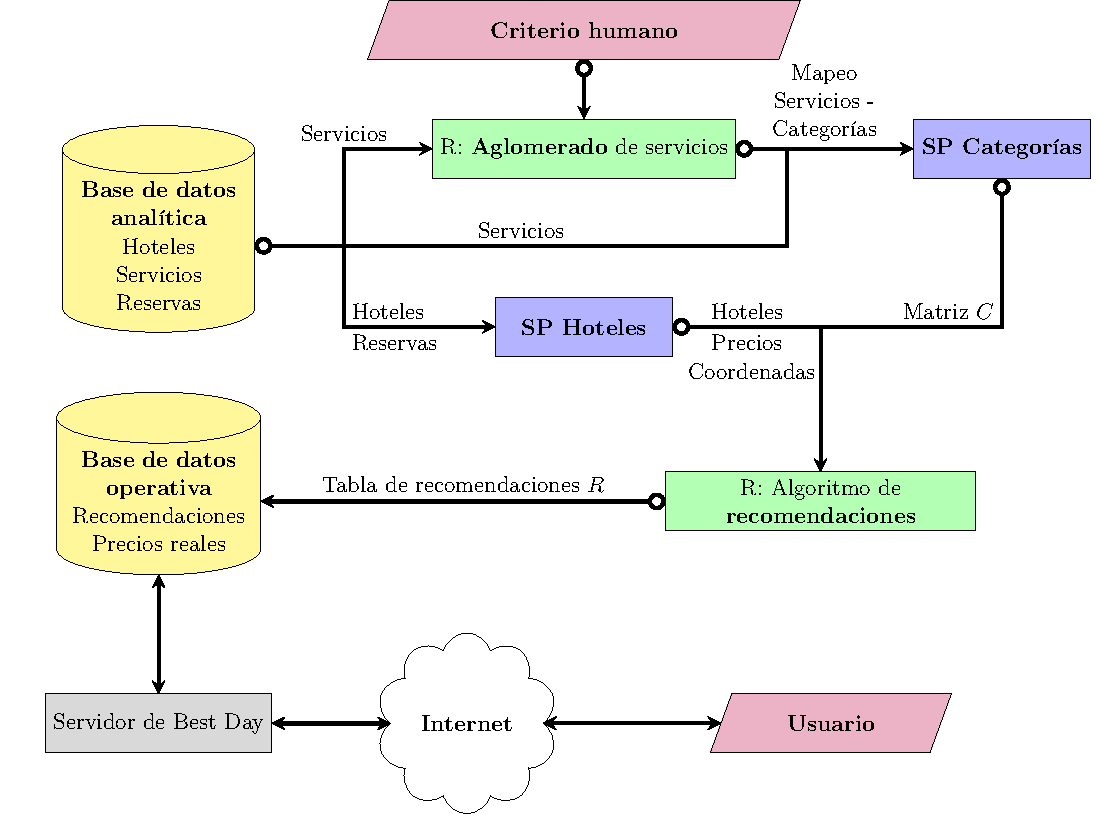
\includegraphics[width=\textwidth]{imagenes/flowchart.pdf}
\end{frame}

%%%%%%%%%%%%%%%%%%%%%%%%%%%%%%%%%%%%%%%%%%%%%%%%%
%%%%%%%%%%%%%%%%%%%%%%%%%%%%%%%%%%%%%%%%%%%%%%%%%
\section{Desempeño}

%%%%%%%%%%%%%%%%%%%%%%%%%%%%%%%%%%%%%%%%%%%%%%%%%
\begin{frame}{Desempeño teórico (antes)}
	\begin{figure}
		\centering
		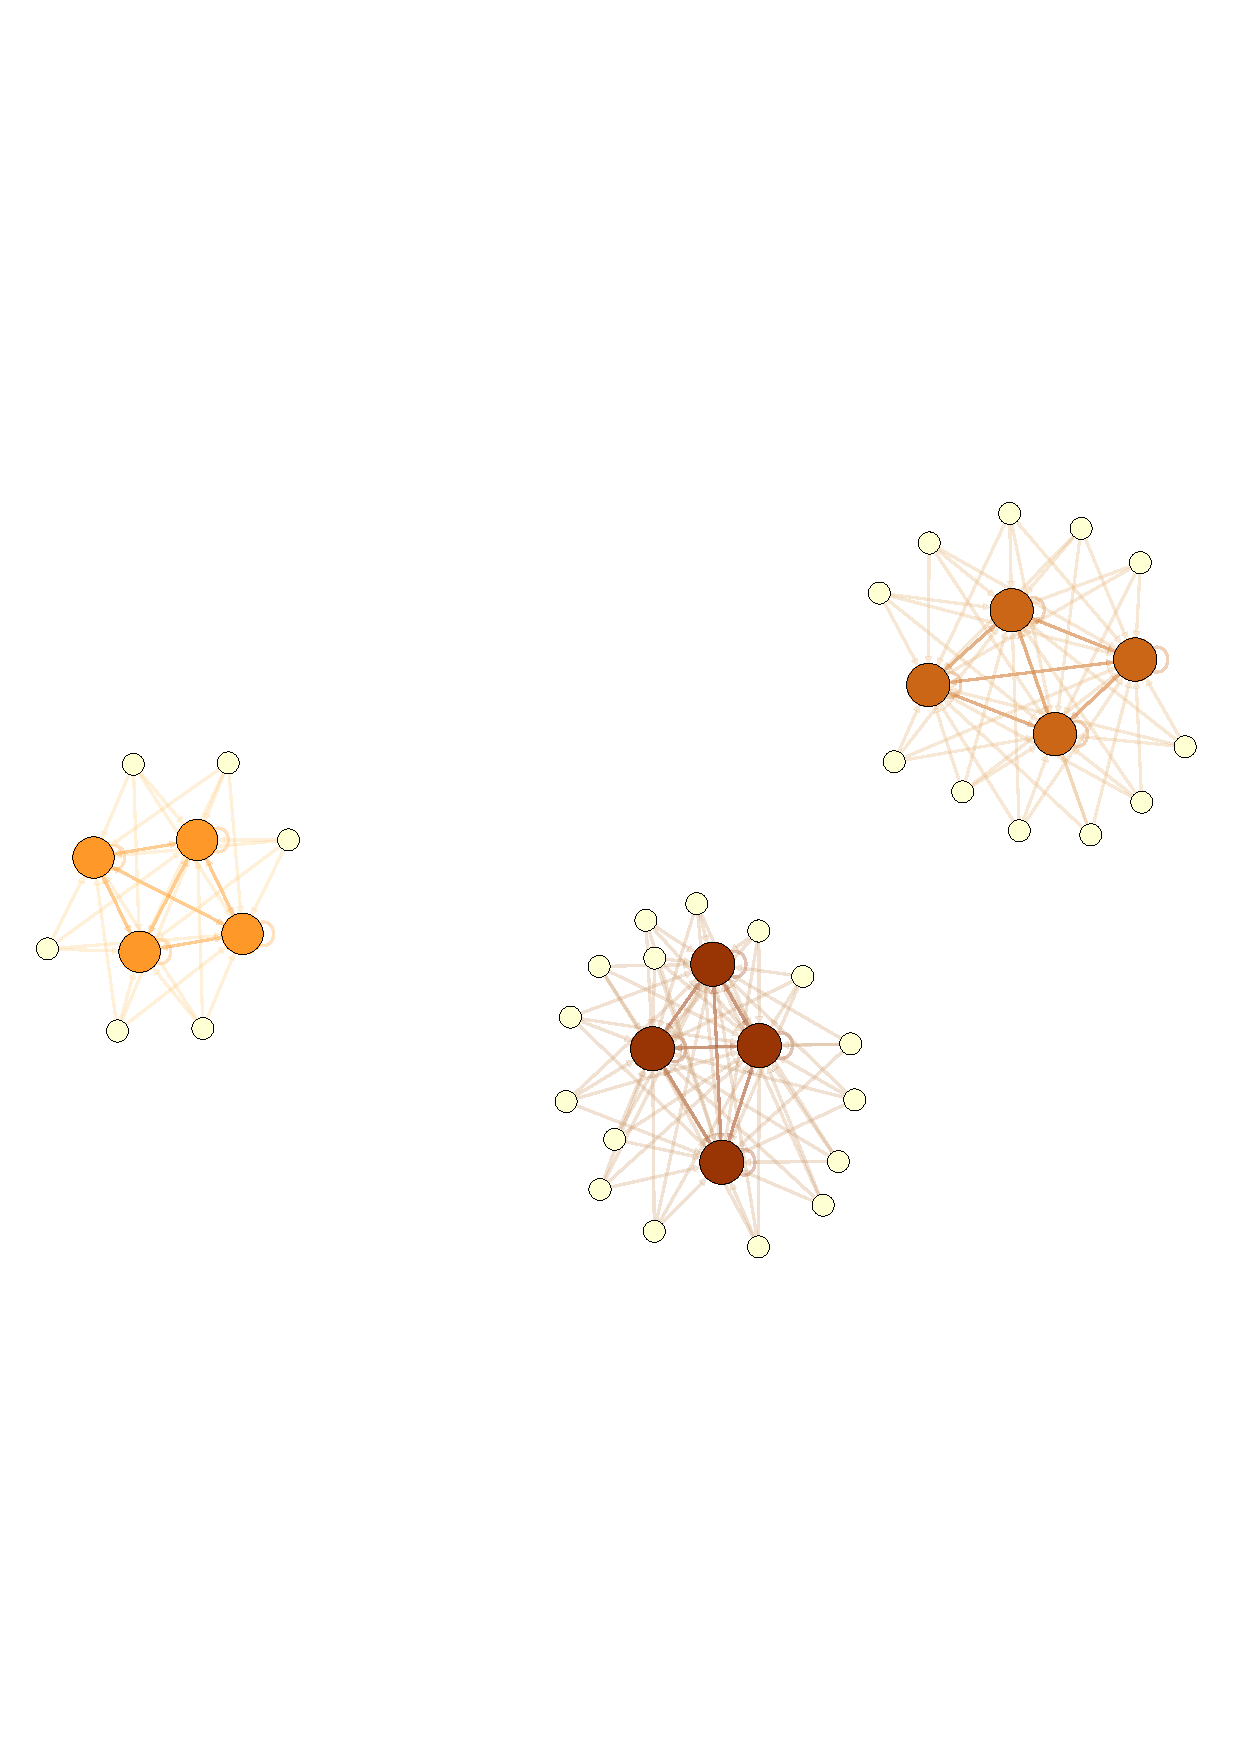
\includegraphics[width=0.6\textwidth, clip = true, trim = 0 0 0 80]{imagenes/disconexo.pdf}
	\end{figure}
\end{frame}

%%%%%%%%%%%%%%%%%%%%%%%%%%%%%%%%%%%%%%%%%%%%%%%%%
\begin{frame}{Desempeño teórico (después)}
	\begin{figure}
		\centering
		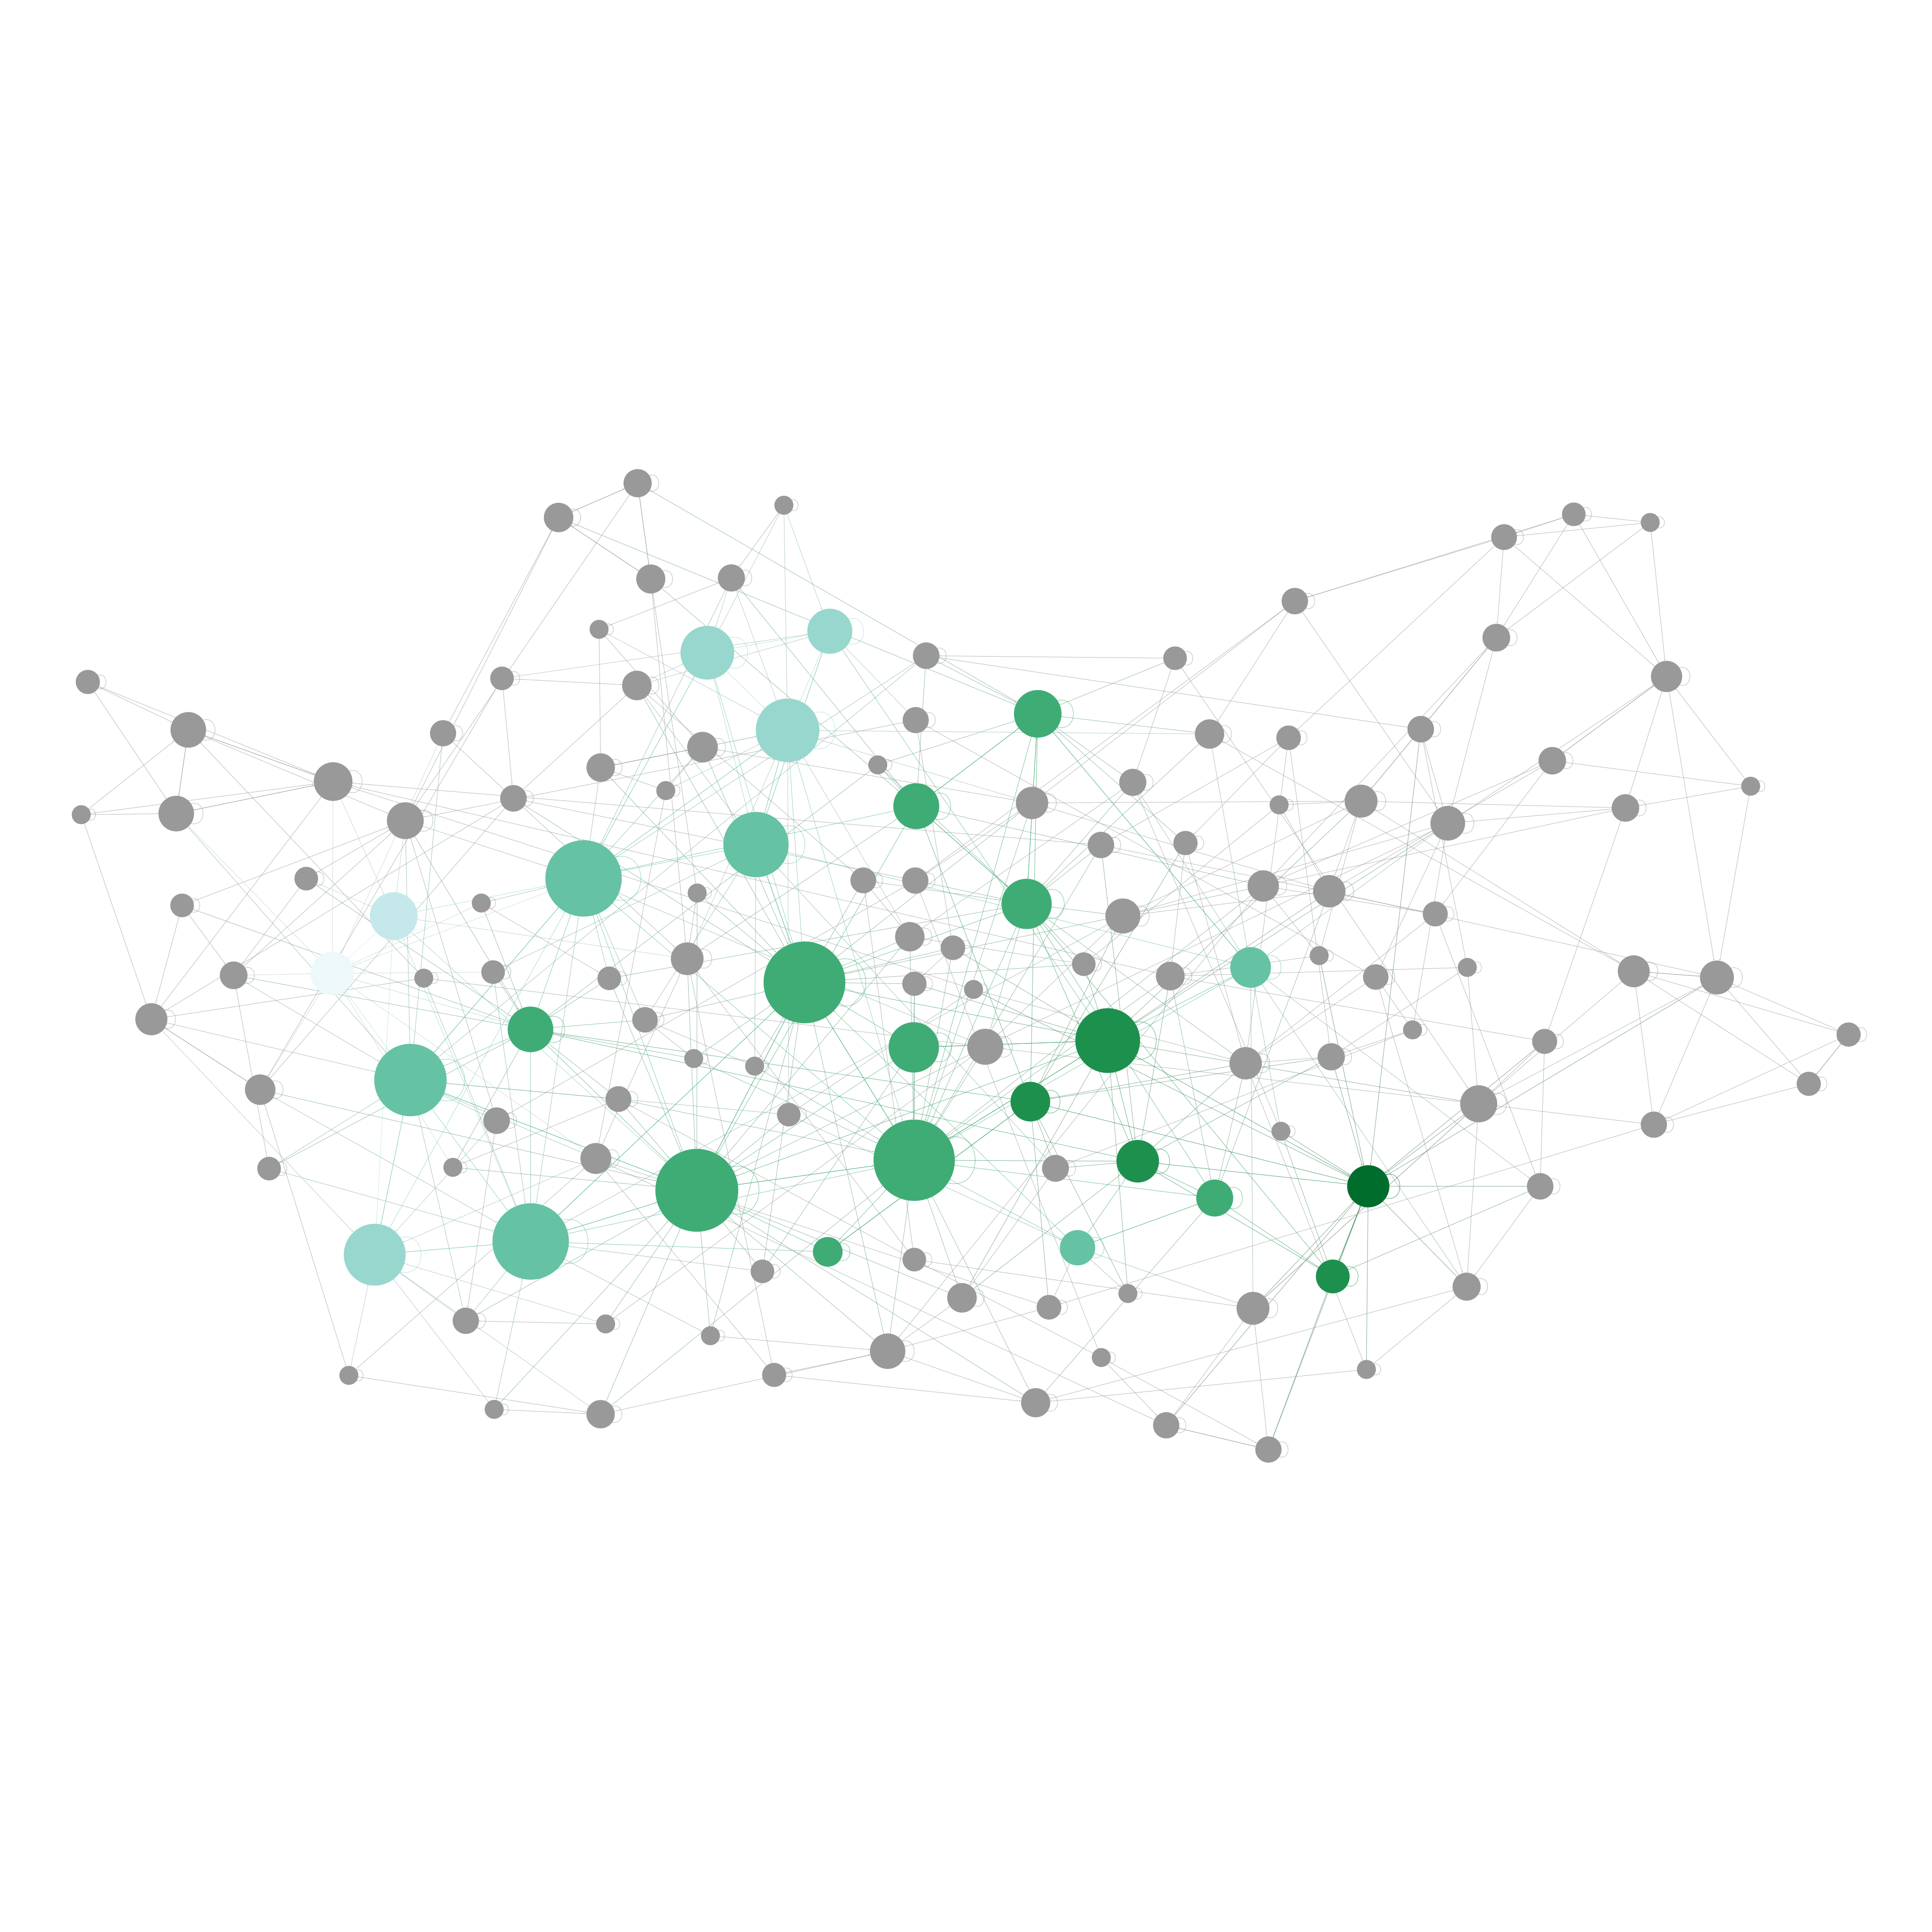
\includegraphics[width=\textwidth, clip = true, trim = 0 0 0 500]{imagenes/cancun_laquinta2.png}
	\end{figure}
\end{frame}

%%%%%%%%%%%%%%%%%%%%%%%%%%%%%%%%%%%%%%%%%%%%%%%%%
\begin{frame}{Desempeño de la página}
	\begin{figure}
		\centering
		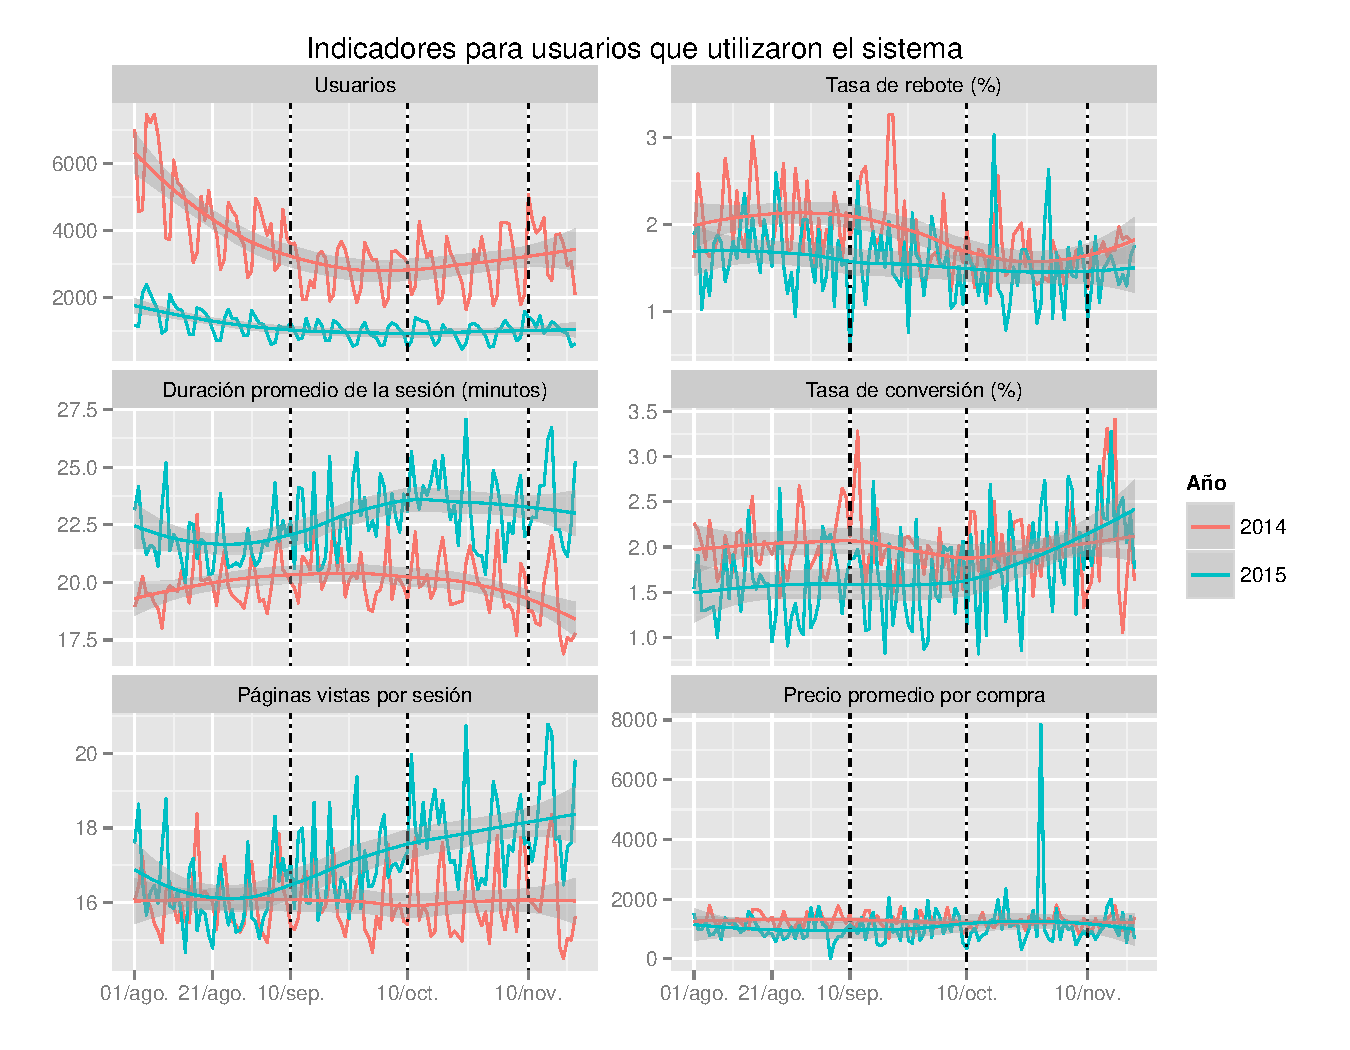
\includegraphics[width=0.85\textwidth]{imagenes/analytics_2015nov23.pdf}
	\end{figure}
\end{frame}

%%%%%%%%%%%%%%%%%%%%%%%%%%%%%%%%%%%%%%%%%%%%%%%%%
\begin{frame}{Conclusiones}
	\begin{itemize}
		\item \textbf{Teóricas:}
		\begin{itemize}
			\item Mejores cualidades: \textbf{precio}, \textbf{distancia}, \textbf{similitud}
			\item La red de recomendaciones está mejor conectada
			\item Mayor \textbf{flexibilidad}: se puede cambiar de categoría gradualmente
		\end{itemize}
		\item \textbf{Prácticas:}
		\begin{itemize}
			\item Impacto importante en los clientes que empezaron a utilizar las recomendaciones
			\item \textbf{Mayor uso} una vez que se utiliza el sistema
			\item Con más tiempo la \textbf{conversión} empezó a aumentar
			\item No hay aumento de entradas (diseño y posición)
		\end{itemize}
		\item \textbf{Trabajo futuro:}
		\begin{itemize}
			\item Precio dinámico, filtro de precio en forma de ``U''
			\item A/B testing
			\item Mayor periodo de observación
		\end{itemize}
	\end{itemize}
\end{frame}

%%%%%%%%%%%%%%%%%%%%%%%%%%%%%%%%%%%%%%%%%%%%%%%%%
\begin{frame}{Anexo: Elección de $\alpha$}
	\centering
	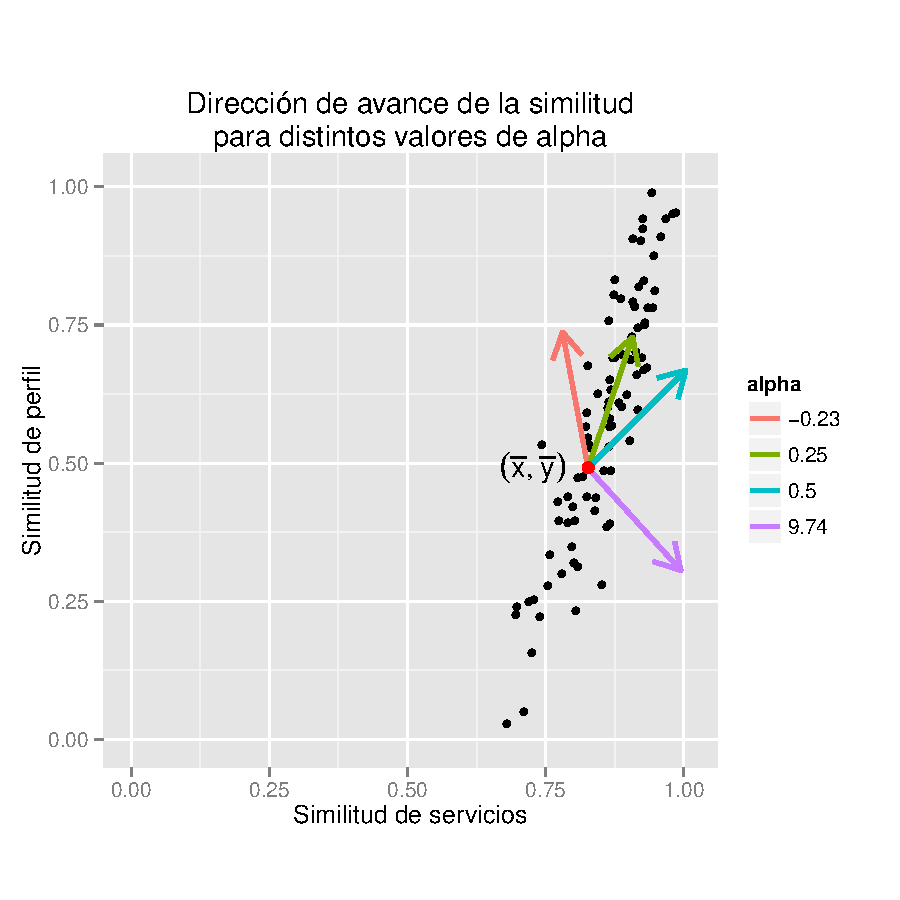
\includegraphics[width=0.75\textwidth]{imagenes/alpha.pdf}
\end{frame}


\end{document} 

















